\documentclass[12pt,a4paper]{article}

\usepackage{amsmath, amssymb, amsthm}
\usepackage{algorithm}
\usepackage{algpseudocode}
\usepackage{graphicx}
\usepackage{tikz}
\usepackage{pgfplots}
\pgfplotsset{compat=1.18}
\usepackage{booktabs}
\usepackage{hyperref}
\usepackage{xcolor}
\usepackage{subcaption}
\usepackage{geometry}
\usepackage{enumitem}
\usepackage{bm}

\geometry{margin=1in}

\usetikzlibrary{arrows.meta, positioning, shapes.geometric, shapes.misc, fit, backgrounds}

\newtheorem{definition}{Definition}
\newtheorem{remark}{Remark}

\title{\textbf{Continual Task Routing via Novelty-Weighted\\Gaussian Mixture Models}}
\author{}
\date{}

\begin{document}

\maketitle

\begin{abstract}
We present a continual learning routing framework that assigns an incoming query to one of a growing set of tasks without retraining earlier task models or retaining their raw training data.
The system maintains a compact \emph{routing space} produced by a frozen pre-trained encoder and a fixed random projection.
For each new task a Gaussian Mixture Model (GMM) is fitted in this shared space; critically, training samples that are already well-explained by existing task densities receive lower weight, concentrating model capacity on genuinely novel regions of the feature space.
At inference, routing is performed by comparing per-task likelihood scores normalized by each task's training statistics.
The approach is entirely non-parametric at the routing level---no gradient-based fine-tuning is required---and adds $\mathcal{O}(M \cdot p)$ storage per new task (where $M$ is the number of mixture components and $p$ the routing dimension).
\end{abstract}

% ─────────────────────────────────────────────────────────────────────────────
\section{Problem Formulation}
\label{sec:problem}
% ─────────────────────────────────────────────────────────────────────────────

Let $\mathcal{T} = \{\mathcal{T}_1, \mathcal{T}_2, \ldots, \mathcal{T}_K\}$ be a sequence of coding tasks (e.g., code translation, bug fixing, code search) that arrive \emph{sequentially}.
Each task $\mathcal{T}_k$ is associated with a training corpus $\mathcal{D}_k = \{x_i^{(k)}\}_{i=1}^{N_k}$ of natural-language prompts.

The goal is to learn a \emph{router} $\mathcal{R} : \mathcal{X} \to \{1,\ldots,K\}$ that, given an unseen query prompt $x$, predicts the task index $k$ it belongs to. The router must satisfy two constraints that are central to continual learning:

\begin{enumerate}[noitemsep]
    \item \textbf{No catastrophic forgetting:} the routing accuracy on $\mathcal{T}_1,\ldots,\mathcal{T}_{k-1}$ must not degrade when $\mathcal{T}_k$ is added.
    \item \textbf{No data retention:} only statistics (GMM parameters), not raw samples, are stored after each task is processed.
\end{enumerate}

% ─────────────────────────────────────────────────────────────────────────────
\section{Routing Feature Extraction}
\label{sec:features}
% ─────────────────────────────────────────────────────────────────────────────

\subsection{Frozen Encoder Backbone}

Let $f_\theta$ be a pre-trained encoder (concretely, CodeT5-small \cite{wang2021codet5}) with $L$ transformer layers and hidden dimension $d$.
All parameters of $f_\theta$ are frozen throughout the entire continual learning process; the encoder serves solely as a fixed feature map.

For a tokenized input sequence of length $T$, the encoder produces a sequence of hidden states $\mathbf{H}^{(\ell)} \in \mathbb{R}^{T \times d}$ for each layer $\ell \in \{0, 1, \ldots, L\}$, where $\ell = 0$ corresponds to the token embedding layer.
We select the representation at layer $\ell^* = \min(\ell_{\mathrm{cfg}}, L)$ with $\ell_{\mathrm{cfg}}$ a hyperparameter (default~4):
\begin{equation}
    \mathbf{H} = \mathbf{H}^{(\ell^*)} \in \mathbb{R}^{T \times d}.
\end{equation}

\subsection{Dual-Pool Representation}

Code generation prompts have a characteristic structure: the \emph{task instruction} (what to do) typically appears in the first tokens, while \emph{contextual code} (relevant snippets) occupies the remainder.
To capture both levels of granularity we construct two pooled vectors.

Let $\mathbf{m} \in \{0,1\}^T$ be the attention mask.
The \emph{masked mean pooling} operator is:
\begin{equation}
    \operatorname{pool}(\mathbf{H}, \mathbf{m}) = \frac{\sum_{t=1}^{T} m_t \, \mathbf{h}_t}{\max\!\left(1,\, \sum_{t=1}^{T} m_t\right)} \in \mathbb{R}^d,
\end{equation}
where $\mathbf{h}_t$ is the $t$-th row of $\mathbf{H}$.

Define the \emph{prefix length} $T_p = \min(64, T)$.
We compute:
\begin{align}
    \mathbf{h}_{\mathrm{prefix}} &= \operatorname{pool}(\mathbf{H}_{1:T_p},\, \mathbf{m}_{1:T_p}) \in \mathbb{R}^d, \label{eq:hprefix} \\
    \mathbf{h}_{\mathrm{full}}   &= \operatorname{pool}(\mathbf{H},\, \mathbf{m}) \in \mathbb{R}^d, \label{eq:hfull}
\end{align}
and concatenate them into a $2d$-dimensional vector:
\begin{equation}
    \tilde{\mathbf{h}} = \left[\mathbf{h}_{\mathrm{prefix}};\, \mathbf{h}_{\mathrm{full}}\right] \in \mathbb{R}^{2d}.
    \label{eq:concat}
\end{equation}

\subsection{Layer Normalization and Random Projection}
\label{sec:proj}

We apply parameter-free Layer Normalization (no learnable scale or shift) to $\tilde{\mathbf{h}}$ to remove scale ambiguity:
\begin{equation}
    \mathbf{h} = \operatorname{LN}(\tilde{\mathbf{h}}) \in \mathbb{R}^{2d}, \qquad
    \operatorname{LN}(\mathbf{v}) = \frac{\mathbf{v} - \mu_{\mathbf{v}}}{\sigma_{\mathbf{v}} + \varepsilon} \cdot \mathbf{1},
    \label{eq:ln}
\end{equation}
where $\mu_\mathbf{v}$ and $\sigma_\mathbf{v}$ are the mean and standard deviation of the elements of $\mathbf{v}$, and $\varepsilon$ is a small numerical stabilizer.

A \emph{fixed} projection matrix $\mathbf{P} \in \mathbb{R}^{p \times 2d}$ ($p \leq 2d$, default $p=256$) reduces dimensionality for efficient density estimation.
The rows of $\mathbf{P}$ are constructed to be orthonormal:

\begin{enumerate}[noitemsep]
    \item Draw $\mathbf{A} \in \mathbb{R}^{2d \times p}$ with $A_{ij} \sim \mathcal{N}(0, 1/p)$ using a fixed random seed.
    \item Compute the thin QR factorization: $\mathbf{A} = \mathbf{Q}\mathbf{R}$, $\mathbf{Q} \in \mathbb{R}^{2d \times p}$.
    \item Set $\mathbf{P} = \mathbf{Q}^\top$ so that $\mathbf{P}\mathbf{P}^\top = \mathbf{I}_p$.
\end{enumerate}

The final routing embedding for a sample $x$ is:
\begin{equation}
    \mathbf{z} = \mathbf{P} \, \mathbf{h} \in \mathbb{R}^p.
    \label{eq:z}
\end{equation}

Since $\mathbf{P}$ is fixed at initialization (from a seeded RNG) and never updated, the routing space is stable across all tasks, which is essential for the GMM densities to remain comparable.

\begin{figure}[t]
\centering
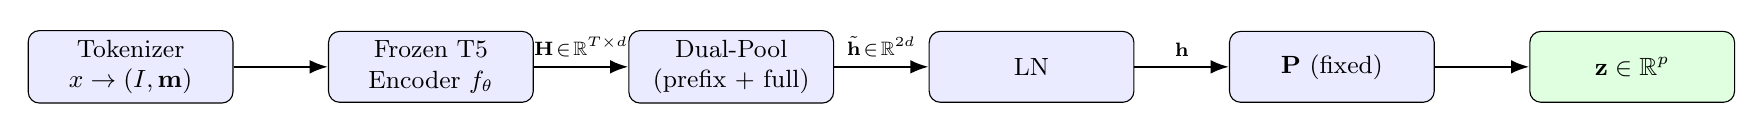
\begin{tikzpicture}[
    box/.style={draw, rounded corners=4pt, minimum width=2.6cm, minimum height=0.9cm,
                align=center, fill=blue!8},
    op/.style={draw, circle, minimum size=0.7cm, fill=orange!20, font=\small},
    arr/.style={-Latex, thick},
    font=\small
]
    \node[box] (tok) {Tokenizer\\$x \to (I,\mathbf{m})$};
    \node[box, right=1.2cm of tok] (enc) {Frozen T5\\Encoder $f_\theta$};
    \node[box, right=1.2cm of enc] (pool) {Dual-Pool\\(prefix + full)};
    \node[box, right=1.2cm of pool] (ln)  {LN};
    \node[box, right=1.2cm of ln]  (proj) {$\mathbf{P}$ (fixed)};
    \node[box, right=1.2cm of proj, fill=green!12] (z) {$\mathbf{z}\in\mathbb{R}^p$};

    \draw[arr] (tok)  -- (enc);
    \draw[arr] (enc)  -- node[above,font=\scriptsize]{$\mathbf{H}\!\in\!\mathbb{R}^{T\times d}$} (pool);
    \draw[arr] (pool) -- node[above,font=\scriptsize]{$\tilde{\mathbf{h}}\!\in\!\mathbb{R}^{2d}$} (ln);
    \draw[arr] (ln)   -- node[above,font=\scriptsize]{$\mathbf{h}$} (proj);
    \draw[arr] (proj) -- (z);
\end{tikzpicture}
\caption{Feature extraction pipeline. All parameters (encoder $f_\theta$ and projection $\mathbf{P}$) are fixed after initialization.}
\label{fig:pipeline}
\end{figure}

% ─────────────────────────────────────────────────────────────────────────────
\section{Weighted Diagonal GMM}
\label{sec:gmm}
% ─────────────────────────────────────────────────────────────────────────────

\subsection{Model Definition}

For each task $k$ we model the distribution of routing embeddings $\{\mathbf{z}_i^{(k)}\}$ as a \emph{diagonal} Gaussian Mixture Model (GMM) with $M$ components:
\begin{equation}
    p_k(\mathbf{z}) = \sum_{m=1}^{M} \pi_m^{(k)} \, \mathcal{N}\!\left(\mathbf{z};\, \bm{\mu}_m^{(k)},\, \operatorname{diag}\!\left(\bm{\sigma}_m^{(k)2}\right)\right),
    \label{eq:gmm}
\end{equation}
where $\pi_m^{(k)} \geq 0$, $\sum_m \pi_m^{(k)} = 1$, and $\bm{\sigma}_m^{(k)2} \in \mathbb{R}^p_{>0}$ are per-dimension variances.
The diagonal covariance assumption is motivated by computational efficiency and regularization: with $p=256$ dimensions, estimating full covariances from limited data ($N \sim 2000$ samples) would be severely ill-conditioned.

The log-likelihood of a single point $\mathbf{z}$ under component $m$ is:
\begin{equation}
    \log \mathcal{N}\!\left(\mathbf{z};\bm{\mu}_m, \bm{\sigma}_m^2\right)
    = -\frac{1}{2}\left[p\ln(2\pi) + \sum_{j=1}^p \ln \sigma_{mj}^2
    + \sum_{j=1}^p \frac{(z_j - \mu_{mj})^2}{\sigma_{mj}^2}\right].
    \label{eq:logN}
\end{equation}
The marginal log-likelihood is computed stably via the log-sum-exp trick:
\begin{equation}
    \log p_k(\mathbf{z}) = \operatorname{logsumexp}_m\!\left[\log\pi_m^{(k)} + \log \mathcal{N}(\mathbf{z};\bm{\mu}_m^{(k)},\bm{\sigma}_m^{(k)2})\right].
    \label{eq:logpk}
\end{equation}

\subsection{Weighted EM Algorithm}
\label{sec:wem}

Let $\mathcal{D}_k = \{(\mathbf{z}_i, w_i)\}_{i=1}^N$ be the weighted training set for task $k$, where $w_i > 0$ are sample weights (detailed in Section~\ref{sec:novelty}).
We maximize the \emph{weighted log-likelihood}:
\begin{equation}
    \mathcal{L}(\bm{\theta}) = \frac{\sum_{i=1}^N w_i \log p_k(\mathbf{z}_i)}{\sum_{i=1}^N w_i},
    \label{eq:wll}
\end{equation}
where $\bm{\theta} = \{\pi_m, \bm{\mu}_m, \bm{\sigma}_m^2\}_{m=1}^M$.

The EM updates in closed form are as follows.

\paragraph{E-step.} Compute the \emph{responsibility} of component $m$ for sample $i$:
\begin{equation}
    r_{im} = \frac{\pi_m \, \mathcal{N}(\mathbf{z}_i;\bm{\mu}_m,\bm{\sigma}_m^2)}{\sum_{m'} \pi_{m'}\,\mathcal{N}(\mathbf{z}_i;\bm{\mu}_{m'},\bm{\sigma}_{m'}^2)}.
    \label{eq:resp}
\end{equation}

\paragraph{M-step.} Compute the \emph{weighted effective count} for component $m$:
\begin{equation}
    \tilde{N}_m = \sum_{i=1}^N w_i \, r_{im}, \qquad \Omega = \sum_{i=1}^N w_i.
    \label{eq:Nk}
\end{equation}
Then update:
\begin{align}
    \pi_m &= \frac{\tilde{N}_m}{\Omega}, \label{eq:pi_update} \\[4pt]
    \bm{\mu}_m &= \frac{\sum_{i=1}^N w_i r_{im} \, \mathbf{z}_i}{\tilde{N}_m}, \label{eq:mu_update} \\[4pt]
    \sigma_{mj}^2 &= \max\!\left(\frac{\sum_{i=1}^N w_i r_{im}(z_{ij}-\mu_{mj})^2}{\tilde{N}_m},\; \sigma^2_{\min}\right), \label{eq:var_update}
\end{align}
where $\sigma^2_{\min} > 0$ is a \emph{variance floor} that prevents numerical collapse of components (default $10^{-4}$).

\paragraph{Convergence criterion.} EM iterates for at most $T_{\max}$ steps (default 50) or until
\begin{equation}
    \left|\mathcal{L}^{(t)} - \mathcal{L}^{(t-1)}\right| < \delta, \quad \delta = 10^{-4}.
    \label{eq:conv}
\end{equation}

\paragraph{Initialization.} Means $\bm{\mu}_m$ are initialized by sampling $M$ data points without replacement, with sampling probabilities proportional to the sample weights $w_i$.
All components share the global (unweighted) per-dimension variance as their initial $\bm{\sigma}_m^2$.
Mixing coefficients are initialized uniformly: $\pi_m = 1/M$.

\begin{algorithm}[t]
\caption{Weighted EM for Diagonal GMM}
\label{alg:wem}
\begin{algorithmic}[1]
\Require Embeddings $\{\mathbf{z}_i\}_{i=1}^N$, weights $\{w_i\}_{i=1}^N$, components $M$, floor $\sigma^2_{\min}$, tol $\delta$, max iters $T_{\max}$
\Ensure GMM parameters $\{\pi_m, \bm{\mu}_m, \bm{\sigma}_m^2\}_{m=1}^M$
\State Initialize $\pi_m, \bm{\mu}_m, \bm{\sigma}_m^2$ as described above
\State $\mathcal{L}^{(0)} \gets -\infty$
\For{$t = 1, \ldots, T_{\max}$}
    \State \textbf{E-step:} compute responsibilities $r_{im}$ via \eqref{eq:resp} using log-sum-exp
    \State \textbf{M-step:} compute $\tilde{N}_m$ via \eqref{eq:Nk}, then update $\pi_m, \bm{\mu}_m, \bm{\sigma}_m^2$ via \eqref{eq:pi_update}--\eqref{eq:var_update}
    \State $\mathcal{L}^{(t)} \gets \bigl(\sum_i w_i \log p(\mathbf{z}_i)\bigr) / \Omega$
    \If{$|\mathcal{L}^{(t)} - \mathcal{L}^{(t-1)}| < \delta$}
        \State \textbf{break}
    \EndIf
\EndFor
\State \Return $\{\pi_m, \bm{\mu}_m, \bm{\sigma}_m^2\}_{m=1}^M$
\end{algorithmic}
\end{algorithm}

% ─────────────────────────────────────────────────────────────────────────────
\section{Continual Task Router}
\label{sec:router}
% ─────────────────────────────────────────────────────────────────────────────

\subsection{Novelty Weighting}
\label{sec:novelty}

When learning the $k$-th task, the router already holds GMMs $\{p_1, \ldots, p_{k-1}\}$ for all preceding tasks.
A sample $\mathbf{z}$ from task $k$ that lies in a region already covered by an existing density brings little new information; up-weighting such samples could cause the new GMM to waste capacity modelling shared content already captured by older tasks.

We therefore assign each training sample a \emph{novelty weight} $w_i \in [\omega_{\min}, 1]$ that is high when the sample is novel relative to existing tasks and low when it is already well-explained.

\paragraph{Normalised scores.}
For task $k' < k$ with GMM parameters $(\bm{\theta}^{(k')}, a_{k'}, b_{k'})$
(the scalars $a_{k'}$ and $b_{k'}$ are defined in Section~\ref{sec:norm}),
the normalized log-likelihood of $\mathbf{z}$ under task $k'$ is:
\begin{equation}
    s_{k'}(\mathbf{z}) = \frac{\log p_{k'}(\mathbf{z}) - a_{k'}}{b_{k'} + \varepsilon}.
    \label{eq:score}
\end{equation}

\paragraph{Coverage.}
The best-matching existing task determines how well $\mathbf{z}$ is already represented:
\begin{equation}
    c(\mathbf{z}) = \max_{k' < k}\; s_{k'}(\mathbf{z}).
    \label{eq:coverage}
\end{equation}

\paragraph{Novelty weight.}
Using a sigmoid to form a smooth indicator of low coverage:
\begin{equation}
    \omega(\mathbf{z}) = \operatorname{clip}\!\left(1 - \sigma\!\left(\frac{c(\mathbf{z}) - \kappa}{\tau_n}\right),\; \omega_{\min},\; 1\right),
    \label{eq:novelty}
\end{equation}
where $\sigma(x) = (1+e^{-x})^{-1}$ is the logistic sigmoid, $\kappa$ is a \emph{coverage threshold} (default $0$), $\tau_n > 0$ is a temperature that controls the sharpness of the transition (default $1.0$), and $\omega_{\min}$ is a minimum weight that prevents any sample from being completely ignored (default $0.05$).

Figure~\ref{fig:novelty} illustrates the novelty weight as a function of normalized coverage.

\begin{figure}[t]
\centering
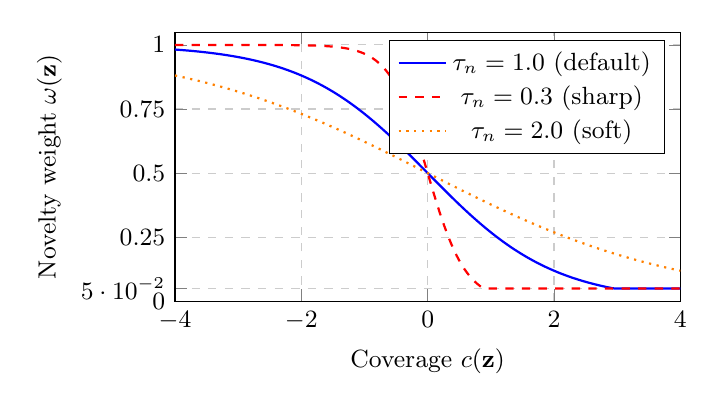
\begin{tikzpicture}
\begin{axis}[
    width=8cm, height=5cm,
    xlabel={Coverage $c(\mathbf{z})$},
    ylabel={Novelty weight $\omega(\mathbf{z})$},
    xmin=-4, xmax=4,
    ymin=0, ymax=1.05,
    ytick={0, 0.05, 0.25, 0.5, 0.75, 1.0},
    grid=major,
    grid style={dashed, gray!40},
    legend pos=north east,
    legend style={font=\small},
    tick label style={font=\small},
    label style={font=\small},
]
\addplot[blue, thick, domain=-4:4, samples=200]
    {max(0.05, min(1.0, 1 - 1/(1 + exp(-x/1.0)))};
\addplot[red, dashed, thick, domain=-4:4, samples=200]
    {max(0.05, min(1.0, 1 - 1/(1 + exp(-x/0.3)))};
\addplot[orange, dotted, thick, domain=-4:4, samples=200]
    {max(0.05, min(1.0, 1 - 1/(1 + exp(-x/2.0)))};
\addlegendentry{$\tau_n=1.0$ (default)}
\addlegendentry{$\tau_n=0.3$ (sharp)}
\addlegendentry{$\tau_n=2.0$ (soft)}
\end{axis}
\end{tikzpicture}
\caption{Novelty weight $\omega(\mathbf{z})$ as a function of coverage $c(\mathbf{z})$ for $\kappa=0$ and three temperatures $\tau_n$. Samples with high coverage (already explained by existing tasks) receive low weight; genuinely novel samples receive weight near 1.}
\label{fig:novelty}
\end{figure}

\subsection{Learning a New Task}

Algorithm~\ref{alg:fit_task} summarises the procedure for incorporating task $k$.

\begin{algorithm}[t]
\caption{Fitting Task $k$ in the Continual Router}
\label{alg:fit_task}
\begin{algorithmic}[1]
\Require Training embeddings $Z_k = \{\mathbf{z}_i^{(k)}\}_{i=1}^N$, existing routers $\{(p_{k'}, a_{k'}, b_{k'})\}_{k'<k}$
\Ensure New task router $(p_k, a_k, b_k)$
\State Compute novelty weights: $w_i \gets \omega(\mathbf{z}_i^{(k)})$ for all $i$ via \eqref{eq:novelty}
\State Fit GMM: $\bm{\theta}^{(k)} \gets \textsc{WeightedEM}(Z_k, \{w_i\}, M)$ \hfill\textit{(Algorithm~\ref{alg:wem})}
\State Compute training log-likelihoods: $\ell_i \gets \log p_k(\mathbf{z}_i^{(k)})$ for all $i$
\State Compute weighted mean: $a_k \gets \dfrac{\sum_i w_i \ell_i}{\Omega}$, $\; \Omega = \sum_i w_i$
\State Compute weighted std: $b_k \gets \sqrt{\dfrac{\sum_i w_i (\ell_i - a_k)^2}{\Omega} + \varepsilon}$
\State Append $(p_k, a_k, b_k)$ to the router registry
\end{algorithmic}
\end{algorithm}

\subsection{Per-Task Score Normalisation}
\label{sec:norm}

Raw log-likelihoods are not directly comparable across tasks: the log-likelihood scale depends on the intrinsic complexity of each task's distribution.
For example, a narrowly concentrated task distribution will have high absolute log-likelihoods, while a diffuse task will yield lower values---even for correctly classified samples.

After fitting the GMM for task $k$, we compute two statistics on the weighted training set:
\begin{align}
    a_k &= \mathbb{E}_w\!\left[\log p_k(\mathbf{z})\right]
         = \frac{\sum_{i=1}^N w_i \log p_k(\mathbf{z}_i^{(k)})}{\Omega},
         \label{eq:ak} \\
    b_k &= \sqrt{\mathrm{Var}_w\!\left[\log p_k(\mathbf{z})\right] + \varepsilon}
         = \sqrt{\frac{\sum_{i=1}^N w_i (\log p_k(\mathbf{z}_i^{(k)}) - a_k)^2}{\Omega} + \varepsilon}.
         \label{eq:bk}
\end{align}
These are the weighted mean and standard deviation of the log-likelihood evaluated on the task's own training data.
At inference, the \emph{normalized score} of a query $\mathbf{z}$ for task $k$ is exactly as defined in \eqref{eq:score}:
\begin{equation}
    s_k(\mathbf{z}) = \frac{\log p_k(\mathbf{z}) - a_k}{b_k + \varepsilon}.
    \label{eq:snorm}
\end{equation}
This is analogous to a $z$-score: it centres the score at zero and scales it by the within-task variability, making scores across different tasks directly comparable.

\subsection{Inference and Routing Decision}

Given a query embedding $\mathbf{z}$, the router computes normalised scores for all $K$ registered tasks and selects the task with the highest score:
\begin{equation}
    \hat{k} = \operatorname*{argmax}_{k \in \{1,\ldots,K\}} \; s_k(\mathbf{z}).
    \label{eq:routing}
\end{equation}
No learned threshold or calibration is required; the routing rule is a pure argmax.

% ─────────────────────────────────────────────────────────────────────────────
\section{Soft Routing Vector}
\label{sec:soft_routing}
% ─────────────────────────────────────────────────────────────────────────────

The normalised GMM scores $s_k(\mathbf{z})$ defined in Section~\ref{sec:norm} serve directly as per-task logits for soft routing.
Rather than taking the argmax (hard routing, \eqref{eq:routing}), we apply a temperature-scaled softmax to obtain a probability distribution over all $K$ tasks:
\begin{equation}
    \alpha_k(x) = \frac{\exp\!\left(s_k(\mathbf{z}) / \tau\right)}{\displaystyle\sum_{j=1}^K \exp\!\left(s_j(\mathbf{z}) / \tau\right)},
    \label{eq:alpha}
\end{equation}
where $\mathbf{z} = \mathbf{P}\operatorname{LN}([\mathbf{h}_{\mathrm{prefix}}; \mathbf{h}_{\mathrm{full}}])$ is the routing embedding from Section~\ref{sec:features} and $\tau > 0$ is a temperature hyperparameter.
The resulting \emph{soft routing vector} is:
\begin{equation}
    \bm{\alpha}(x) = \bigl[\alpha_1(x),\, \ldots,\, \alpha_K(x)\bigr]^\top \in \Delta^{K-1},
    \label{eq:alpha_vec}
\end{equation}
where $\Delta^{K-1}$ denotes the $(K{-}1)$-dimensional probability simplex.

The temperature $\tau$ continuously interpolates between two extreme behaviours:
\begin{itemize}[noitemsep]
    \item $\tau \to 0^+$: $\bm{\alpha}(x) \to \mathbf{e}_{\hat{k}}$, recovering the hard argmax routing of \eqref{eq:routing}.
    \item $\tau \to \infty$: $\bm{\alpha}(x) \to \mathbf{1}/K$, yielding a uniform mixture over all task experts.
\end{itemize}
In practice, $\tau$ is tuned so that the routing distribution is sharp enough to preserve task-specific behaviour yet smooth enough to gracefully handle queries that lie near the boundary between tasks.

\begin{remark}
The same $z$-normalised scores that drive the hard routing decision during continual training are reused for soft routing at inference time.
No additional parameters or re-training are required to switch from hard to soft mode---only $\tau$ changes.
\end{remark}

% ─────────────────────────────────────────────────────────────────────────────
\section{Expert Mixture at Output Distribution Level}
\label{sec:expert_mix}
% ─────────────────────────────────────────────────────────────────────────────

Each task $k$ is associated with a dedicated generative \emph{expert}---concretely, a task-specific LoRA adapter layered on top of a shared frozen backbone---which induces a conditional token distribution:
\begin{equation}
    p_k(y_t \mid x, y_{<t}) = \mathrm{Expert}_k(x, y_{<t}),
    \label{eq:pk}
\end{equation}
where $y_t$ is the output token at step $t$ and $y_{<t}$ is the previously generated prefix.

The final token distribution is the soft mixture of all expert distributions weighted by the soft routing vector:
\begin{equation}
    p_{\mathrm{mix}}(y_t \mid x, y_{<t}) = \sum_{k=1}^K \alpha_k(x)\, p_k(y_t \mid x, y_{<t}).
    \label{eq:pmix}
\end{equation}
Because the routing weights $\alpha_k(x)$ depend only on the input $x$ and not on the generated prefix $y_{<t}$, the routing decision is made \emph{once per query} and remains fixed throughout autoregressive decoding.

\paragraph{Distribution-level vs.\ weight-level mixing.}
Equation~\eqref{eq:pmix} mixes output token \emph{distributions}, not model parameters.
Weight-level merging (e.g.\ $\Delta\mathbf{W}(x)=\sum_k\alpha_k\mathbf{B}_k\mathbf{A}_k$) approximates the mixture by averaging low-rank deltas, discarding cross-adapter interaction effects.
Distribution-level mixing is exact under the mixture-of-experts assumption and preserves full task-specific computation in each expert.
The trade-off is that distribution-level mixing requires $K$ independent expert forward passes per decoding step, while weight-level merging amortises to a single forward pass after fusion.

\paragraph{Autoregressive generation.}
At each decoding step $t$, the vocabulary logits from all $K$ experts are computed in parallel, converted to per-expert probability vectors, linearly combined with $\bm{\alpha}(x)$, and the resulting $p_{\mathrm{mix}}$ is used by beam search:
\begin{equation}
    \hat{y} = \operatorname*{argmax}_{y} \sum_{t=1}^{|y|} \log p_{\mathrm{mix}}(y_t \mid x, y_{<t}).
    \label{eq:generation}
\end{equation}

Algorithm~\ref{alg:generation} gives the complete procedure.

\begin{algorithm}[t]
\caption{Soft-Routing Expert-Mixture Generation}
\label{alg:generation}
\begin{algorithmic}[1]
\Require Query $x$; normalised GMM scores $\{s_k(\mathbf{z})\}$ from \eqref{eq:snorm}; experts $\{E_k\}_{k=1}^K$; temperature $\tau$; beams $B$
\Ensure Generated output $\hat{y}$
\State $\alpha_k \gets \exp(s_k(\mathbf{z})/\tau)/\sum_j\exp(s_j(\mathbf{z})/\tau)$, $\forall k$ \hfill\textit{soft routing; \eqref{eq:alpha}}
\While{decoding not finished}
    \For{$k = 1, \ldots, K$} \textbf{in parallel}
        \State $\ell_k \gets \log E_k(x, y_{<t})$ \Comment{log-logits from expert $k$}
    \EndFor
    \State $\log p_{\mathrm{mix}} \gets \log\!\sum_k \alpha_k \exp(\ell_k)$ \hfill\textit{logsumexp mixture; \eqref{eq:pmix}}
    \State Advance $B$ beams using $\log p_{\mathrm{mix}}$ as next-token log-probability
\EndWhile
\State \Return highest-scoring beam $\hat{y}$
\end{algorithmic}
\end{algorithm}

% ─────────────────────────────────────────────────────────────────────────────
\section{Full System Architecture}
\label{sec:architecture}
% ─────────────────────────────────────────────────────────────────────────────

\begin{figure}[t]
\centering
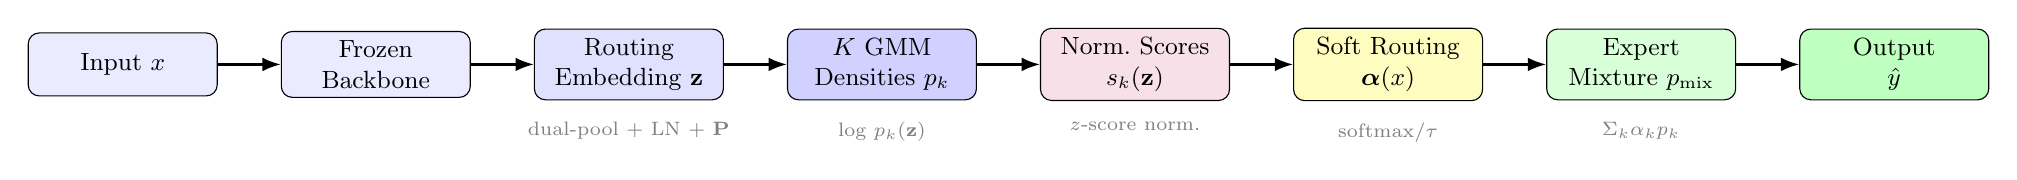
\begin{tikzpicture}[
    font=\small,
    box/.style={draw, rounded corners=4pt, minimum width=2.4cm, minimum height=0.8cm, align=center, fill=blue!8},
    sbox/.style={draw, rounded corners=4pt, minimum width=2.4cm, minimum height=0.8cm, align=center},
    arr/.style={-Latex, thick},
]

\node[box] (x) {Input $x$};
\node[box, right=0.8cm of x] (enc) {Frozen\\Backbone};
\node[sbox, right=0.8cm of enc, fill=blue!12] (z) {Routing\\Embedding $\mathbf{z}$};
\node[sbox, right=0.8cm of z, fill=blue!18] (gmm) {$K$ GMM\\Densities $p_k$};
\node[sbox, right=0.8cm of gmm, fill=purple!12] (sk) {Norm.\ Scores\\$s_k(\mathbf{z})$};
\node[sbox, right=0.8cm of sk, fill=yellow!25] (alpha) {Soft Routing\\$\bm{\alpha}(x)$};
\node[sbox, right=0.8cm of alpha, fill=green!15] (mix) {Expert\\Mixture $p_{\mathrm{mix}}$};
\node[sbox, right=0.8cm of mix, fill=green!25] (out) {Output\\$\hat{y}$};

\draw[arr] (x)    -- (enc);
\draw[arr] (enc)  -- (z);
\draw[arr] (z)    -- (gmm);
\draw[arr] (gmm)  -- (sk);
\draw[arr] (sk)   -- (alpha);
\draw[arr] (alpha)-- (mix);
\draw[arr] (mix)  -- (out);

\node[font=\scriptsize, gray, below=0.15cm of z]     {dual-pool + LN + $\mathbf{P}$};
\node[font=\scriptsize, gray, below=0.15cm of gmm]   {log $p_k(\mathbf{z})$};
\node[font=\scriptsize, gray, below=0.15cm of sk]    {$z$-score norm.};
\node[font=\scriptsize, gray, below=0.15cm of alpha] {softmax$/\tau$};
\node[font=\scriptsize, gray, below=0.15cm of mix]   {$\Sigma_k\alpha_k p_k$};

\end{tikzpicture}
\caption{End-to-end inference pipeline. The frozen backbone encodes input $x$ and the dual-pool aggregation (Section~\ref{sec:features}) yields the routing embedding $\mathbf{z}$. Each of the $K$ task GMMs evaluates the log-density $\log p_k(\mathbf{z})$, which is $z$-score normalised to produce comparable scores $s_k(\mathbf{z})$ (Section~\ref{sec:norm}). A temperature-scaled softmax converts these into soft routing weights $\bm{\alpha}(x)$ (Section~\ref{sec:soft_routing}), which are used to mix the $K$ expert output distributions into $p_{\mathrm{mix}}$ for beam-search decoding (Section~\ref{sec:expert_mix}).}
\label{fig:arch}
\end{figure}

The architecture has two key properties.
First, the backbone and projection are frozen for the lifetime of the system, so no feature drift occurs as tasks accumulate.
Second, the routing operates entirely in the GMM density space---there are no auxiliary branches, and the same normalised scores that drive hard routing during continual training are reused directly for soft routing at inference.

% ─────────────────────────────────────────────────────────────────────────────
\section{Continual Learning Protocol}
\label{sec:cl}
% ─────────────────────────────────────────────────────────────────────────────

The full continual training loop is described in Algorithm~\ref{alg:cl}.

\begin{algorithm}[t]
\caption{Continual Routing Training}
\label{alg:cl}
\begin{algorithmic}[1]
\Require Task sequence $\mathcal{T}_1, \ldots, \mathcal{T}_K$; frozen encoder $f_\theta$; projection $\mathbf{P}$; hyperparameters
\Ensure Trained router with $K$ task GMMs
\State Initialize empty router registry $\mathcal{R} \gets \varnothing$
\For{$k = 1, \ldots, K$}
    \State \textbf{Extract features:} $Z_k \gets \{\mathbf{z}_i^{(k)} = \mathbf{P}\operatorname{LN}([\mathbf{h}^{(k)}_{\mathrm{prefix}};\mathbf{h}^{(k)}_{\mathrm{full}}])\}_{i=1}^{N_k}$
    \State \textbf{Fit task:} $(p_k, a_k, b_k) \gets \textsc{FitNewTask}(Z_k, \mathcal{R})$  \hfill\textit{(Algorithm~\ref{alg:fit_task})}
    \State $\mathcal{R} \gets \mathcal{R} \cup \{(p_k, a_k, b_k)\}$
    \State \textbf{Evaluate:} compute routing accuracy on all seen tasks $\mathcal{T}_1,\ldots,\mathcal{T}_k$
    \State Checkpoint $\mathcal{R}$ to disk
\EndFor
\end{algorithmic}
\end{algorithm}

\paragraph{Feature caching.}
Since the encoder and projection are frozen, features $Z_k$ need to be computed only once per task and split, and can be reloaded in subsequent runs.
This makes ablation studies and hyperparameter search inexpensive.

\paragraph{Evaluation.}
After each task is registered, routing accuracy is measured on held-out evaluation splits of all previously seen tasks.
The confusion matrix $C \in \mathbb{Z}^{k \times k}$ is reported, where $C_{ij}$ counts how many samples truly from task $i$ were routed to task $j$.
Per-task accuracy $\mathrm{acc}_k = C_{kk}/\sum_j C_{kj}$ and macro-average accuracy $\bar{\mathrm{acc}} = \frac{1}{k}\sum_{k'=1}^k \mathrm{acc}_{k'}$ are the primary metrics.

% ─────────────────────────────────────────────────────────────────────────────
\section{Design Choices and Analysis}
\label{sec:analysis}
% ─────────────────────────────────────────────────────────────────────────────

\subsection{Why Diagonal GMMs?}

A full-covariance GMM with $p=256$ dimensions and $M=4$ components requires estimating $M \cdot p(p+1)/2 = 33{,}024$ parameters, compared to only $M \cdot p = 512$ for the diagonal variant.
With typical training budgets of $N=2000$ samples per task, the full-covariance estimator is heavily underdetermined.
The diagonal assumption is equivalent to assuming that, in the projected routing space, feature dimensions are conditionally independent given the component identity---a reasonable approximation given that the orthonormal projection $\mathbf{P}$ decorrelates directions.

\subsection{Role of the Variance Floor}

The variance floor $\sigma^2_{\min}$ in \eqref{eq:var_update} prevents the EM algorithm from converging to degenerate solutions where a single component collapses onto a single data point, sending the log-likelihood to $+\infty$.
It also provides implicit regularization: components cannot become narrower than $\sqrt{\sigma^2_{\min}}$ in any dimension, preventing overfitting to small clusters.

\subsection{Novelty Weight Interpretation}

The novelty weight $\omega(\mathbf{z}_i)$ in \eqref{eq:novelty} can be interpreted as an importance sampling weight that reweights the training distribution of task $k$ to emphasise the \emph{residual} distribution---the part of $\mathcal{D}_k$ not already captured by earlier tasks.
This is reminiscent of boosting and residual density estimation, but applied in the continual learning setting where earlier models cannot be retrained.

\begin{remark}
When $\kappa = 0$ and a sample has coverage $c(\mathbf{z}) = 0$ (meaning it is at the boundary of existing task distributions), its novelty weight is $\omega = 1 - \sigma(0) = 0.5$. The threshold $\kappa$ can be tuned to shift this operating point: negative $\kappa$ makes the router more aggressive in down-weighting samples that are only mildly covered.
\end{remark}

\subsection{Score Normalisation and Inter-Task Comparability}

Without normalisation, the argmax routing rule in \eqref{eq:routing} would be biased towards tasks whose distributions happen to have higher absolute log-likelihoods (e.g., more concentrated or lower-dimensional effective distributions).
The $z$-score normalisation in \eqref{eq:snorm} ensures that each task's score distribution has zero mean and unit variance on its own training data, making the competition between tasks fair.

\paragraph{Connection to likelihood ratio testing.}
Note that the unnormalised score $\log p_k(\mathbf{z})$ is a log-likelihood.
The normalised score $s_k(\mathbf{z})$ can be viewed as a standardised test statistic for the hypothesis $H_0: \mathbf{z} \sim p_k$.
Routing then selects the task whose null hypothesis is least rejected.

\subsection{Complexity Summary}

Table~\ref{tab:complexity} summarises the per-task cost of each stage.

\begin{table}[t]
\centering
\caption{Per-task computational complexity. $N$ = training samples, $B$ = batch size, $T$ = sequence length, $d$ = encoder hidden size, $p$ = routing dimension, $M$ = GMM components, $T_{\max}$ = EM iterations, $K$ = tasks seen so far.}
\label{tab:complexity}
\begin{tabular}{llll}
\toprule
Stage & Time & Memory (params) & Notes \\
\midrule
\multicolumn{4}{l}{\textit{Training: feature extraction and density fitting}} \\
\midrule
Feature extraction   & $\mathcal{O}(N B^{-1} T d L)$    & $\mathcal{O}(|f_\theta|)$     & Frozen backbone, no grad \\
Projection           & $\mathcal{O}(N \cdot d \cdot r)$  & $\mathcal{O}(dr)$             & Fixed task-local basis $\mathbf{U}_k$ \\
Novelty weights      & $\mathcal{O}(N K)$                & ---                           & $K$ normalised-score evals \\
EM fitting           & $\mathcal{O}(T_{\max} N M r)$     & $\mathcal{O}(NMr)$            & Main training bottleneck \\
GMM storage/task     & ---                               & $\mathcal{O}(Mr^2 + Mr)$      & $M$ Gaussians in $\mathbb{R}^r$ \\
\midrule
\multicolumn{4}{l}{\textit{Inference: routing and generation}} \\
\midrule
GMM score (density)  & $\mathcal{O}(K M r)$              & $\mathcal{O}(KMr)$            & Per query \\
Soft routing softmax & $\mathcal{O}(K)$                  & ---                           & Per query \\
Expert mixture       & $\mathcal{O}(K \cdot |y| \cdot |f_0|)$ & $\mathcal{O}(K|f_0|)$   & $K$ forward passes/step \\
\bottomrule
\end{tabular}
\end{table}

% ─────────────────────────────────────────────────────────────────────────────
\section{Hyperparameter Summary}
\label{sec:hyperparams}
% ─────────────────────────────────────────────────────────────────────────────

\begin{table}[h]
\centering
\caption{Hyperparameters and their default values.}
\label{tab:hyperparams}
\begin{tabular}{lll}
\toprule
Symbol & Name & Default \\
\midrule
\multicolumn{3}{l}{\textit{Feature extraction and density fitting}} \\
\midrule
$\ell_{\mathrm{cfg}}$ & Feature layer index & 4 \\
$p$ & Routing dimension (GMM space) & 256 \\
$r$ & Task-local density dimension & 32 \\
$M$ & GMM components per task & 4 \\
$T_{\max}$ & Max EM iterations & 50 \\
$\delta$ & EM convergence tolerance & $10^{-4}$ \\
$\sigma^2_{\min}$ & Variance floor & $10^{-4}$ \\
$\varepsilon$ & Numerical stabiliser & $10^{-8}$ \\
$\kappa$ & Coverage threshold (novelty) & 0.0 \\
$\tau_n$ & Novelty sigmoid temperature & 1.0 \\
$\omega_{\min}$ & Minimum novelty weight & 0.05 \\
$T_p$ & Prefix pool length (tokens) & 64 \\
$N_{\mathrm{train}}$ & Training samples per task & 2000 \\
$N_{\mathrm{eval}}$ & Evaluation samples per task & 1000 \\
\midrule
\multicolumn{3}{l}{\textit{Soft routing and expert mixture (Sections~\ref{sec:soft_routing}--\ref{sec:expert_mix})}} \\
\midrule
$\tau$ & Softmax routing temperature & 1.0 \\
$B$ & Beam search width & 4 \\
\bottomrule
\end{tabular}
\end{table}

% ─────────────────────────────────────────────────────────────────────────────
\section{Summary}
\label{sec:summary}
% ─────────────────────────────────────────────────────────────────────────────

We have described an end-to-end continual routing and generation system built on a single GMM density branch.
The key components are:
\begin{enumerate}
    \item \textbf{Routing feature extraction (Section~\ref{sec:features}).}
          A frozen backbone with dual-pool aggregation and a fixed QR-orthonormal projection yields stable, task-discriminative routing embeddings $\mathbf{z} \in \mathbb{R}^p$.
          No gradient updates to the backbone are ever needed.

    \item \textbf{Continual GMM fitting (Sections~\ref{sec:gmm}--\ref{sec:router}).}
          For each new task, a diagonal GMM is fitted in the routing space via novelty-weighted EM.
          Novelty weights down-weight samples already well-explained by earlier tasks, focusing the new GMM on the residual distribution.
          Per-task $z$-score normalisation ensures that log-density scores are directly comparable across all $K$ tasks.

    \item \textbf{Soft routing vector (Section~\ref{sec:soft_routing}).}
          At inference time, the normalised GMM scores $\{s_k(\mathbf{z})\}_{k=1}^K$ are passed through a temperature-scaled softmax to produce a proper routing distribution $\bm{\alpha}(x)\in\Delta^{K-1}$ over task experts.
          The temperature $\tau$ smoothly interpolates between hard argmax routing ($\tau\to 0$) and uniform mixing ($\tau\to\infty$).

    \item \textbf{Expert mixture at output level (Section~\ref{sec:expert_mix}).}
          Each task expert (a task-specific LoRA adapter on the frozen backbone) produces an independent token distribution.
          The final distribution $p_{\mathrm{mix}} = \sum_k \alpha_k p_k$ is the routing-weighted mixture, which is exact under the mixture-of-experts assumption and preserves full task-specific computation.
\end{enumerate}
Together, these four components form a pipeline that accumulates new tasks without modifying earlier modules, routes entirely through the GMM density model, and enables both hard (argmax) and soft (temperature-weighted) task selection---all without any task-identity label at test time.



\bibliographystyle{plainnat}
\begin{thebibliography}{9}

\bibitem{wang2021codet5}
Y. Wang, W. Wang, S. Joty, and S. C. H. Hoi.
\newblock CodeT5: Identifier-aware Unified Pre-trained Encoder-Decoder Models for Code Understanding and Generation.
\newblock In \emph{Proceedings of EMNLP}, 2021.

\bibitem{dempster1977maximum}
A. P. Dempster, N. M. Laird, and D. B. Rubin.
\newblock Maximum likelihood from incomplete data via the EM algorithm.
\newblock \emph{Journal of the Royal Statistical Society, Series B}, 39(1):1--38, 1977.

\bibitem{reynolds2009gaussian}
D. A. Reynolds.
\newblock Gaussian Mixture Models.
\newblock \emph{Encyclopedia of Biometrics}, 741:659--663, 2009.

\bibitem{kirkpatrick2017overcoming}
J. Kirkpatrick et al.
\newblock Overcoming catastrophic forgetting in neural networks.
\newblock \emph{Proceedings of the National Academy of Sciences}, 114(13):3521--3526, 2017.

\bibitem{johnson1984extensions}
W. B. Johnson and J. Lindenstrauss.
\newblock Extensions of Lipschitz mappings into a Hilbert space.
\newblock \emph{Contemporary Mathematics}, 26:189--206, 1984.

\bibitem{jacobs1991adaptive}
R. A. Jacobs, M. I. Jordan, S. J. Nowlan, and G. E. Hinton.
\newblock Adaptive mixtures of local experts.
\newblock \emph{Neural Computation}, 3(1):79--87, 1991.

\bibitem{shazeer2017outrageously}
N. Shazeer, A. Mirhoseini, K. Maziarz, A. Davis, Q. V. Le, G. E. Hinton, and J. Dean.
\newblock Outrageously Large Neural Networks: The Sparsely-Gated Mixture-of-Experts Layer.
\newblock In \emph{Proceedings of ICLR}, 2017.

\bibitem{shalev2011online}
S. Shalev-Shwartz.
\newblock Online Learning and Online Convex Optimization.
\newblock \emph{Foundations and Trends in Machine Learning}, 4(2):107--194, 2011.

\end{thebibliography}

\end{document}
